\documentclass[10pt]{standalone}
%\usepackage[utf8]{inputenc}
\usepackage{pgfplots}
\pgfplotsset{compat=1.15}
\usepackage{mathrsfs}
\usetikzlibrary{arrows}
\pagestyle{empty}
\begin{document}

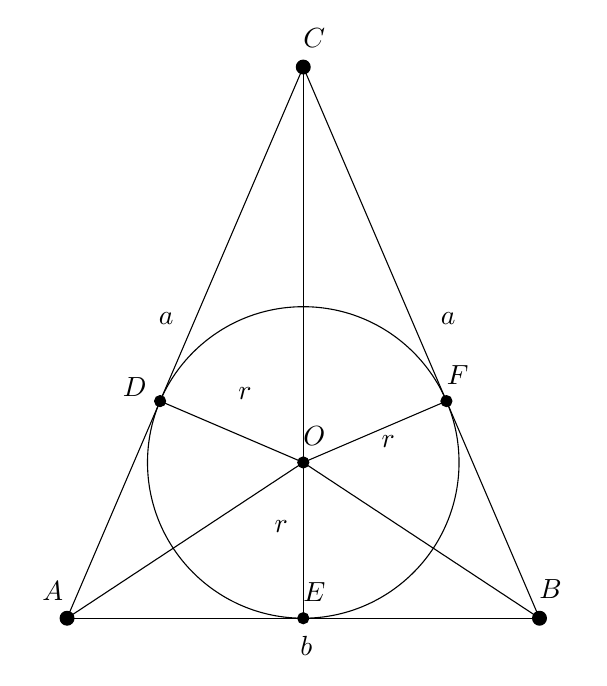
\begin{tikzpicture}[line cap=round,line join=round,>=triangle 45,x=1.0cm,y=1.0cm]
%%\begin{axis}[
%x=1.0cm,y=1.0cm,
%axis lines=middle,
%ymajorgrids=true,
%xmajorgrids=true,
%xmin=1.5,
%xmax=8.5,
%ymin=-0.5,
%ymax=7.5,
%xtick={2.0,3.0,...,8.0},
%ytick={-0.0,1.0,...,7.0},]
\clip(1.5,-0.5) rectangle (8.5,7.5);
\draw  (2.,0.)-- (8.,0.);
\draw  (2.,0.)-- (5.,1.9781884739416735);
\draw  (8.,0.)-- (5.,7.);
\draw  (8.,0.)-- (5.,1.9781884739416735);
\draw  (5.,7.)-- (2.,0.);
\draw  (5.,1.9781884739416735)-- (6.818242104262498,2.757435090054173);
\draw  (5.,1.9781884739416735)-- (3.1817578957375026,2.7574350900541718);
\draw  (5.,1.9781884739416735)-- (5.,0.);
\draw  (5.,1.9781884739416749) circle (1.9781884739416755cm);
\draw  (5.,7.)-- (5.,0.);
\draw [fill=black] (2.,0.) circle (2.5pt);
\draw[color=black] (1.82,0.35) node {$A$};
\draw [fill=black] (8.,0.) circle (2.5pt);
\draw[color=black] (8.14,0.37) node {$B$};
\draw [fill=black] (5.,7.) circle (2.5pt);
\draw[color=black] (5.14,7.37) node {$C$};
\draw[color=black] (5.04,-0.35) node {$b$};
\draw[color=black] (6.84,3.81) node {$a$};
\draw[color=black] (3.26,3.81) node {$a$};
\draw [fill=black] (5.,1.9781884739416735) circle (2.0pt);
\draw[color=black] (5.14,2.31) node {$O$};
\draw [fill=black] (3.1817578957375026,2.7574350900541718) circle (2.0pt);
\draw[color=black] (2.86,2.93) node {$D$};
\draw [fill=black] (6.818242104262498,2.757435090054173) circle (2.0pt);
\draw[color=black] (6.96,3.09) node {$F$};
\draw[color=black] (6.08,2.25) node {$r$};
\draw[color=black] (4.26,2.85) node {$r$};
\draw [fill=black] (5.,0.) circle (2.0pt);
\draw[color=black] (5.14,0.33) node {$E$};
\draw[color=black] (4.72,1.17) node {$r$};

%\end{axis}
\end{tikzpicture}
\end{document}